\section{Introduction}
\label{sec:introduction}

Modern academic collaborations increasingly rely on distributed laboratory infrastructures in which students and faculty must securely share private web applications, telemetry, and naming services across institutional boundaries. Within Module~2 of the \textit{Sistemas de Comunicaci\'{o}n~2} course, a Collaborative Online International Learning (COIL) partnership between Universidad de los Llanos (Villavicencio, Meta, Colombia) and Seneca Polytechnic (Toronto, Ontario, Canada) requires interconnecting geographically separated hosts so that participants at each institution can navigate cultural intranet portals deployed by their counterparts.

Directly exposing local development servers across residential and campus networks introduces severe architectural obstacles, including symmetric Network Address Translation (NAT), carrier-grade address sharing, restrictive campus firewalls, and ephemeral public IPv4 leases \cite{tanenbaum2021,kurose2017}. Furthermore, relying on raw IP addresses, unencrypted HTTP transport, or untrusted self-signed certificates degrades usability and fails enterprise security baselines. To overcome these limitations without dedicated site-to-site VPN hardware, COIL Group~2 engineered a unified Software-Defined Wide Area Network (SD-WAN) overlay coupled with a private Public Key Infrastructure (PKI), authoritative DNS resolution, and packet-level forensic validation \cite{zerotier2024}.

The implementation satisfies four measurable engineering objectives:
\begin{enumerate}
    \item \textbf{Private SD-WAN Overlay Interconnection:} Deploy a cryptographically authenticated ZeroTier Layer-2/Layer-3 overlay network over the \texttt{172.22.0.0/16} subnet with an interface Maximum Transmission Unit (MTU) of \qty{1300}{\byte}, strict private admission (\num{5}/\num{10} authorized endpoints, zero unauthorized hosts), explicit student and server labeling, and verified peer-to-peer ICMP reachability \cite{zerotier2024}.
    \item \textbf{Dual Cultural Intranets under HTTPS/TLS~1.3 with Custom Root CA Trust:} Serve responsive institutional cultural intranets for Universidad de los Llanos and Seneca Polytechnic over HTTPS (TLS~1.3) backed by a custom Root Certificate Authority (\texttt{COIL Group 2 Root CA}) installed in client operating system trust stores to eliminate browser security warnings (rubric bonus criterion).
    \item \textbf{Authoritative DNS Domain Resolution:} Operate an authoritative UDP port~53 DNS service resolving institutional project domains (\texttt{www.coil-group2.com} and subdomains) across the SD-WAN mesh while forwarding external queries upstream, eliminating manual IP-based access.
    \item \textbf{Wireshark Packet Forensics ($< \qty{10}{\mega\byte}$):} Capture live HTTPS client-server traffic over the ZeroTier virtual interface into a compact \texttt{.pcapng} trace strictly below \qty{10}{\mega\byte}, verifying TCP three-way handshakes, TLS~1.3 negotiation and encrypted payload delivery, and graceful connection teardowns.
\end{enumerate}

The remainder of this report documents the ZeroTier SD-WAN IP allocation and verification evidence (Rubric Section~I), individual English-narrated demonstration videos (Rubric Section~II), Wireshark packet dissection (Rubric Section~III), step-by-step deployment manuals covering SD-WAN, web hosting, PKI trust, and DNS resolution (Rubric Section~IV), and concluding quantitative findings alongside the complete project source code in the appendices.

\section{ZeroTier SD-WAN IP Assignment and Node Labeling}
\label{sec:zerotier_sdwan}

Addressing Rubric Section~I (\qty{5}{\percent}), this section presents the overlay network architecture, the complete authorized node registry, compliance with student and web-server labeling rules, and empirical reachability measurements across desktop and mobile endpoints. Step-by-step provisioning commands and controller configuration workflows are deferred to Manual~1 in Section~IV to avoid procedural duplication.

\subsection{SD-WAN Overlay Architecture and Addressing Plan}
\label{subsec:sdwan_architecture}

ZeroTier abstracts physical WAN diversity into a flat virtual Ethernet broadcast domain by decoupling the underlay transport (Virtual Layer~1, VL1) from virtualized switching and addressing (Virtual Layer~2, VL2) \cite{zerotier2024}. Each endpoint generates a cryptographic public/private key pair whose hash forms a unique 40-bit (10-hexadecimal-character) Node ID, enabling authenticated UDP encapsulation and NAT hole punching across disparate residential ISPs without central traffic hairpins \cite{zerotier2024,kurose2017}.

For the COIL Group~2 deployment, the private overlay network ``COIL Group 2 SD-WAN - UniLlanos \& Seneca'' was provisioned under Network ID \texttt{abfd31bd47affa39} with \textit{Private} access control enabled, ensuring that packets from unapproved endpoints are dropped at the controller plane. All authorized interfaces operate on the managed IPv4 prefix \texttt{172.22.0.0/16} with a virtual interface MTU of \qty{1300}{\byte}. Selecting a \qty{1300}{\byte} overlay MTU provides sufficient headroom beneath standard \qty{1500}{\byte} physical Ethernet and PPPoE underlay links to accommodate VL1 UDP/cryptographic encapsulation overhead without outer IP fragmentation \cite{tanenbaum2021,zerotier2024}. At the time of verification, the network held \num{5}/\num{10} included device slots, comprising \num{5} authorized nodes and \num{0} unauthorized nodes (\num{3} active desktop hosts and \num{2} inactive mobile devices).

\begin{figure*}[htbp]
\centering
\definecolor{ztInk}{HTML}{0F172A}
\definecolor{ztMuted}{HTML}{475569}
\definecolor{ztCtrlBg}{HTML}{F5F0FF}
\definecolor{ztCtrlLine}{HTML}{6D28D9}
\definecolor{ztCtrlDark}{HTML}{4C1D95}
\definecolor{ztUniBg}{HTML}{EFF6FF}
\definecolor{ztUniLine}{HTML}{1D4ED8}
\definecolor{ztUniDark}{HTML}{1E3A8A}
\definecolor{ztSenBg}{HTML}{ECFDF5}
\definecolor{ztSenLine}{HTML}{047857}
\definecolor{ztSenDark}{HTML}{064E3B}
\definecolor{ztCliBg}{HTML}{FFF7ED}
\definecolor{ztCliLine}{HTML}{C2410C}
\definecolor{ztCliDark}{HTML}{7C2D12}
\definecolor{ztSumBg}{HTML}{F8FAFC}
\definecolor{ztSumLine}{HTML}{64748B}
\definecolor{ztMeshLine}{HTML}{334155}

\resizebox{0.96\textwidth}{!}{%
\begin{tikzpicture}[
    >=Stealth,
    zone box/.style={
        draw=#1, line width=0.85pt, dashed, rounded corners=6pt, inner sep=6pt
    },
    zone hdr/.style={
        font=\scriptsize\bfseries, text=#1, inner xsep=2pt, inner ysep=1.5pt
    },
    card frame/.style={
        draw=#1, line width=0.85pt, rounded corners=4pt, inner sep=4pt, fill=white
    },
    card pill/.style={
        fill=#1, text=white, font=\scriptsize\bfseries,
        rounded corners=2.5pt, inner xsep=5pt, inner ysep=3pt, align=flush left
    },
    card body/.style={
        font=\fontsize{6.8}{9.2}\selectfont, text=ztInk, align=flush left,
        inner xsep=3pt, inner ysep=2.5pt
    },
    p2p link/.style={
        {Stealth[length=5pt,width=4pt]}-{Stealth[length=5pt,width=4pt]},
        line width=1.35pt, shorten >=1.5pt, shorten <=1.5pt
    },
    mesh stub/.style={
        -{Stealth[length=4.5pt,width=3.5pt]},
        line width=1.0pt, color=ztMeshLine, shorten >=1.5pt, shorten <=0pt
    },
    ctrl link/.style={
        -{Stealth[length=4.5pt,width=3.5pt]},
        line width=0.85pt, densely dashed, color=ztCtrlLine,
        rounded corners=4pt, shorten >=1.5pt, shorten <=1pt
    },
    edge badge/.style={
        draw=#1, fill=white, line width=0.65pt, rounded corners=3pt,
        font=\fontsize{6.4}{8.6}\selectfont, text=ztInk, align=center,
        inner xsep=4pt, inner ysep=3pt
    },
    ctrl tag/.style={
        fill=white, text=ztCtrlDark, font=\fontsize{6}{8.0}\selectfont\bfseries,
        inner xsep=3pt, inner ysep=1.5pt, rounded corners=2pt
    }
]

\node[card pill=ztUniDark, text width=4.65cm, anchor=north west] (n1_hdr) at (0,0)
    {Node 1: UniLlanos Primary Host};
\node[card body, text width=4.65cm, below=2pt of n1_hdr.south, anchor=north] (n1_body) {%
    \textbf{Miguel Rodriguez - Unillanos Website Server}\\
    ID: \texttt{AED30A4FDD} (\texttt{aed30a4fdd})\\
    OS: Windows 11 (\texttt{x86\_64})\\
    ZeroTier IP: \texttt{172.22.201.2/16}\\
    Physical IP: \texttt{181.51.34.123}\\
    Services: \texttt{server\_https.py} (TCP \texttt{443} TLS 1.3 \& TCP \texttt{80}),
    \texttt{dns\_server.py} (UDP \texttt{53}), Private Root CA (\texttt{COIL Group 2 Root CA})%
};
\begin{pgfonlayer}{cardbg}
    \node[card frame=ztUniLine, fit=(n1_hdr)(n1_body)] (node1) {};
\end{pgfonlayer}
\node[zone hdr=ztUniDark, anchor=south west] (uni_hdr) at ($(node1.north west) + (0, 3pt)$)
    {UNILLANOS HOST ZONE};
\begin{pgfonlayer}{zonebg}
    \node[zone box=ztUniLine, fill=ztUniBg, fit=(uni_hdr)(node1)] (uni_zone) {};
\end{pgfonlayer}

\node[card pill=ztCliDark, text width=4.15cm, below=2.9cm of node1.south west, anchor=north west] (n3_hdr)
    {Node 3: Partner Student PC};
\node[card body, text width=4.15cm, below=2pt of n3_hdr.south, anchor=north] (n3_body) {%
    \textbf{Luis Alejandro Leon - Student Client}\\
    ID: \texttt{B63D8AEBA8} (\texttt{b63d8aeba8})\\
    OS: Windows (\texttt{x86\_64})\\
    ZeroTier IPs: \texttt{172.22.100.11}, \texttt{172.22.164.74}\\
    Physical IP: \texttt{181.51.34.104}%
};

\node[card pill=ztCliDark, text width=3.8cm, right=0.55cm of n3_hdr.north east, anchor=north west] (n4_hdr)
    {Node 4: Partner Mobile Client};
\node[card body, text width=3.8cm, below=2pt of n4_hdr.south, anchor=north] (n4_body) {%
    \textbf{Luis Alejandro Leon - Student Client}\\
    ID: \texttt{F6FCD4CE4D} (\texttt{f6fcd4ce4d})\\
    OS: Android (\texttt{arm64})\\
    ZeroTier IP: \texttt{172.22.100.10}%
};

\node[card pill=ztCliDark, text width=4.15cm, right=0.55cm of n4_hdr.north east, anchor=north west] (n5_hdr)
    {Node 5: Mobile Verification Client};
\node[card body, text width=4.15cm, below=2pt of n5_hdr.south, anchor=north] (n5_body) {%
    \textbf{Miguel Rodriguez - Student Client}\\
    ID: \texttt{8EB3130D2C} (\texttt{8eb3130d2c})\\
    OS: Android (\texttt{arm64})\\
    ZeroTier IPs: \texttt{172.22.38.108}, \texttt{172.22.201.50}%
};

\path let \p1=(n3_body.south), \p2=(n4_body.south), \p3=(n5_body.south) in
    coordinate (cli_bot) at (0, {min(\y1, min(\y2, \y3))});
\begin{pgfonlayer}{cardbg}
    \node[card frame=ztCliLine, fit=(n3_hdr)(n3_body)(n3_hdr |- cli_bot)] (node3) {};
    \node[card frame=ztCliLine, fit=(n4_hdr)(n4_body)(n4_hdr |- cli_bot)] (node4) {};
    \node[card frame=ztCliLine, fit=(n5_hdr)(n5_body)(n5_hdr |- cli_bot)] (node5) {};
\end{pgfonlayer}
\node[zone hdr=ztCliDark, anchor=south west] (cli_hdr) at ($(node3.north west) + (0, 3pt)$)
    {REMOTE CLIENTS ZONE};
\begin{pgfonlayer}{zonebg}
    \node[zone box=ztCliLine, fill=ztCliBg, fit=(cli_hdr)(node3)(node4)(node5)] (cli_zone) {};
\end{pgfonlayer}

\node[card pill=ztSenDark, text width=4.65cm, anchor=north east] (n2_hdr) at (n1_hdr.north -| n5_hdr.east)
    {Node 2: Seneca Partner Gateway};
\node[card body, text width=4.65cm, below=2pt of n2_hdr.south, anchor=north] (n2_body) {%
    \textbf{Seneca College - Simulated Gateway}\\
    ID: \texttt{1C84E39095} (\texttt{1c84e39095})\\
    OS: Windows 11 (\texttt{x86\_64})\\
    ZeroTier IP: \texttt{172.22.31.69/16}\\
    Physical IP: \texttt{181.51.34.123}\\
    Services: \texttt{server\_https.py} (TCP \texttt{443} TLS 1.3 \& TCP \texttt{80})\\
    Hosts: Seneca Intranet (\texttt{/seneca/})%
};
\path let \p1=(n1_body.south), \p2=(n2_body.south) in
    coordinate (srv_bot) at (0, {min(\y1, \y2)});
\begin{pgfonlayer}{cardbg}
    \node[card frame=ztSenLine, fit=(n2_hdr)(n2_body)(n2_hdr |- srv_bot)] (node2) {};
\end{pgfonlayer}
\node[zone hdr=ztSenDark, anchor=south west] (sen_hdr) at ($(node2.north west) + (0, 3pt)$)
    {SENECA GATEWAY ZONE};
\begin{pgfonlayer}{zonebg}
    \node[zone box=ztSenLine, fill=ztSenBg, fit=(sen_hdr)(node2)] (sen_zone) {};
\end{pgfonlayer}

\node[card body, text width=7.95cm, anchor=south west] (ctrl_c_body) at ($(node1.west |- uni_zone.north) + (0, 1.05cm)$) {%
    \textbf{Network ID:} \texttt{abfd31bd47affa39} \;\textbar\; \textbf{Subnet:} \texttt{172.22.0.0/16} \;\textbar\; \textbf{MTU:} \qty{1300}{\byte}\\
    \textbf{Overlay Transport:} Virtual Ethernet L2/L3 Mesh over UDP port \texttt{9993}%
};
\node[card pill=ztCtrlDark, text width=7.95cm, anchor=south] (ctrl_c_hdr) at ($(ctrl_c_body.north) + (0, 2pt)$)
    {ZeroTier Central Controller (\texttt{my.zerotier.com})};

\node[card pill=ztCtrlDark, text width=4.65cm, anchor=north east] (ctrl_p_hdr) at (ctrl_c_hdr.north -| n2_hdr.east)
    {Planet Root Servers};
\node[card body, text width=4.65cm, below=2pt of ctrl_p_hdr.south, anchor=north] (ctrl_p_body) {%
    \textbf{Root IDs:} \texttt{778cde7190}, \texttt{cafe80ed74}\\
    Peer Discovery, NAT Traversal \& Relay%
};

\path let \p1=(ctrl_c_body.south), \p2=(ctrl_p_body.south) in
    coordinate (ctrl_bot) at (0, {min(\y1, \y2)});
\begin{pgfonlayer}{cardbg}
    \node[card frame=ztCtrlLine, fit=(ctrl_c_hdr)(ctrl_c_body)(ctrl_c_hdr |- ctrl_bot)] (ctrl_central) {};
    \node[card frame=ztCtrlLine, fit=(ctrl_p_hdr)(ctrl_p_body)(ctrl_p_hdr |- ctrl_bot)] (ctrl_planet) {};
\end{pgfonlayer}
\node[zone hdr=ztCtrlDark, anchor=south west] (ctrl_hdr) at ($(ctrl_central.north west) + (0, 3pt)$)
    {CONTROL PLANE \& UNDERLAY DISCOVERY};
\begin{pgfonlayer}{zonebg}
    \node[zone box=ztCtrlLine, fill=ztCtrlBg, fit=(ctrl_hdr)(ctrl_central)(ctrl_planet)] (ctrl_zone) {};
\end{pgfonlayer}

\coordinate (top_mid) at ($(ctrl_zone.north west)!0.5!(ctrl_zone.north east)$);
\node[font=\normalsize\bfseries, text=ztInk, anchor=south] (figtitle) at ($(top_mid) + (0, 0.38cm)$)
    {COIL Group 2 ZeroTier SD-WAN Overlay Topology};

\coordinate (c_n1_x) at ($(n1_hdr.north east) - (0.65cm, 0)$);
\draw[ctrl link] (ctrl_zone.south -| c_n1_x) -- (node1.north -| c_n1_x);
\node[ctrl tag] at ($(ctrl_zone.south -| c_n1_x)!0.5!(uni_zone.north -| c_n1_x)$) {Auth \& Config};

\coordinate (c_n2_x) at ($(n2_hdr.north east) - (0.65cm, 0)$);
\draw[ctrl link] (ctrl_zone.south -| c_n2_x) -- (node2.north -| c_n2_x);
\node[ctrl tag] at ($(ctrl_zone.south -| c_n2_x)!0.5!(sen_zone.north -| c_n2_x)$) {Auth \& Key Dist.};

\coordinate (ctrl_rail_x) at ($(sen_zone.east) + (0.45cm, 0)$);
\draw[ctrl link] (ctrl_zone.east) -- (ctrl_zone.east -| ctrl_rail_x) |- (cli_zone.east);
\node[ctrl tag, align=center] at ($(ctrl_rail_x |- sen_zone.south)!0.5!(ctrl_rail_x |- cli_zone.north)$)
    {Control /\\[1pt]STUN};

\coordinate (lan_mid) at ($(node1.east)!0.5!(node2.west)$);
\draw[p2p link, color=ztSenLine] (node1.east) -- (node2.west);
\node[edge badge=ztSenLine, above=5pt of lan_mid, anchor=south, text width=3.15cm] (lan_top) {%
    \textbf{LAN ZeroTier P2P}\\
    \texttt{192.168.10.x:9993}%
};
\node[edge badge=ztSenLine, below=5pt of lan_mid, anchor=north, text width=3.15cm] (lan_bot) {%
    ICMP avg: \qty{10}{\milli\second} (rev. \qty{6}{\milli\second})\\
    DNS latency: \qty{0.53}{\milli\second}%
};

\coordinate (wan_x) at ($(node3.north east) - (0.35cm, 0)$);
\draw[p2p link, color=ztUniLine] (node1.south -| wan_x) -- (node3.north -| wan_x);
\coordinate (wan_mid) at ($(uni_zone.south -| wan_x)!0.5!(cli_zone.north -| wan_x)$);
\node[edge badge=ztUniLine, left=5pt of wan_mid, anchor=east, text width=3.65cm] (wan_lbl) {%
    \textbf{WAN ZeroTier P2P} (\texttt{181.51.34.104:20594})\\
    ICMP avg: \qty{31}{\milli\second} / \qty{23}{\milli\second} (\qty{0}{\percent} loss)%
};

\coordinate (mesh_y) at ($(uni_zone.south)!0.50!(cli_zone.north)$);
\coordinate (mesh_x1) at ($(node1.south east) - (0.30cm, 0)$);
\coordinate (mesh_x4) at (node4.north);
\coordinate (mesh_x5) at (node5.north);

\draw[line width=1.1pt, color=ztMeshLine] (mesh_x1 |- mesh_y) -- (mesh_x5 |- mesh_y);
\foreach \mx in {mesh_x1, mesh_x4, mesh_x5} {
    \fill[ztMeshLine] (\mx |- mesh_y) circle (1.7pt);
}
\draw[mesh stub] (mesh_x1 |- mesh_y) -- (node1.south -| mesh_x1);
\draw[mesh stub] (mesh_x5 |- mesh_y) -- (node2.south -| mesh_x5);
\draw[mesh stub] (mesh_x4 |- mesh_y) -- (node4.north);
\draw[mesh stub] (mesh_x5 |- mesh_y) -- (node5.north);

\node[edge badge=ztMeshLine, text width=4.3cm] at ($(mesh_x4 |- mesh_y)!0.5!(mesh_x5 |- mesh_y)$) {%
    \textbf{Virtual Ethernet L2/L3 Mesh}\\
    \texttt{172.22.0.0/16} \textbar\ UDP \texttt{9993} \textbar\ MTU \qty{1300}{\byte}%
};

\path let \p1=(cli_zone.west), \p2=(cli_zone.east) in
    node[draw=ztSumLine, fill=ztSumBg, rounded corners=4pt, inner xsep=6pt, inner ysep=5pt,
         text width={(\x2-\x1)-12.85pt}, align=center,
         font=\fontsize{6.6}{9.5}\selectfont, text=ztInk, anchor=north west]
    (sum_bar) at ($(cli_zone.south west) + (0, -0.32cm)$) {%
        {\fontsize{6.6}{9.6}\selectfont
        \textbf{Verified Overlay Summary:}~
        Network \texttt{abfd31bd47affa39} (\texttt{172.22.0.0/16}, MTU \qty{1300}{\byte})
        \;\textbar\;
        \textbf{LAN P2P:} \qty{10}{\milli\second} / rev. \qty{6}{\milli\second}, DNS \qty{0.53}{\milli\second}\\[2pt]
        \textbf{WAN P2P:} \qty{31}{\milli\second} / \qty{23}{\milli\second} (\qty{0}{\percent} loss)
        \;\textbar\;
        \textbf{Security Stack:} TLS 1.3 (TCP \texttt{443}) + \texttt{COIL Group 2 Root CA}\par}%
    };

\matrix[ampersand replacement=\&, below=0.22cm of sum_bar.south, anchor=north, column sep=7pt, inner sep=0pt,
        nodes={font=\fontsize{6.5}{8.6}\selectfont, text=ztMuted, inner sep=1pt, anchor=west}] (legend_mat) {
    \node[font=\fontsize{6.5}{8.6}\selectfont\bfseries, text=ztInk] {Legend:}; \&
    \node[draw=ztCtrlLine, fill=ztCtrlBg, minimum width=0.28cm, minimum height=0.22cm, rounded corners=1pt] {}; \&
    \node {Control Plane}; \&
    \node[draw=ztUniLine, fill=ztUniBg, minimum width=0.28cm, minimum height=0.22cm, rounded corners=1pt] {}; \&
    \node {UniLlanos Host}; \&
    \node[draw=ztSenLine, fill=ztSenBg, minimum width=0.28cm, minimum height=0.22cm, rounded corners=1pt] {}; \&
    \node {Seneca Gateway}; \&
    \node[draw=ztCliLine, fill=ztCliBg, minimum width=0.28cm, minimum height=0.22cm, rounded corners=1pt] {}; \&
    \node {Remote Clients}; \&
    \node[minimum width=0.45cm, minimum height=0.2cm] (leg_c) {}; \&
    \node {Control Signaling}; \&
    \node[minimum width=0.45cm, minimum height=0.2cm] (leg_p) {}; \&
    \node {P2P / Mesh Link}; \\
};
\draw[ctrl link, shorten >=0pt, shorten <=0pt] (leg_c.west) -- (leg_c.east);
\draw[p2p link, color=ztSenLine, shorten >=0pt, shorten <=0pt] (leg_p.west) -- (leg_p.east);

\end{tikzpicture}%
}
\caption{COIL Group 2 ZeroTier SD-WAN overlay network architecture (\texttt{abfd31bd47affa39}, \texttt{172.22.0.0/16}, MTU \qty{1300}{\byte}). The control plane (\texttt{my.zerotier.com} and Planet root servers) coordinates cryptographic authorization and NAT traversal over UDP/9993, interconnecting the UniLlanos primary server (\texttt{172.22.201.2}), the Seneca Polytechnic gateway (\texttt{172.22.31.69}), and partner desktop/mobile clients.}
\label{fig:sdwan_topology}
\end{figure*}


As illustrated in Fig.~\ref{fig:sdwan_topology}, the virtual \texttt{172.22.0.0/16} switching fabric logically unifies the UniLlanos multi-tenant HTTPS and authoritative DNS host (\texttt{172.22.201.2/16}), the simulated Seneca Polytechnic gateway (\texttt{172.22.31.69/16}), and the remote student desktop and Android clients across physical WAN boundaries.

\subsection{Authorized Member Registry and Node Labeling Compliance}
\label{subsec:member_registry}

Rubric Section~I mandates that every group member connect a host to the SD-WAN, that each node carry an explicit label bearing the corresponding student's name, and that the web server host explicitly declare its hosting role. Table~\ref{tab:zerotier_members} compiles the authoritative registry of all five enrolled endpoints observed in ZeroTier Central.

\begin{table*}[t]
\centering
\caption{ZeroTier Central Authorized Member Registry for Network \texttt{abfd31bd47affa39} (\texttt{COIL Group 2 SD-WAN - UniLlanos \& Seneca}).}
\label{tab:zerotier_members}
\resizebox{\textwidth}{!}{%
\begin{tabular}{@{}lllllll@{}}
\toprule
\textbf{Node ID / Virtual MAC} & \textbf{Assigned Label / Role} & \textbf{OS / Arch (Client)} & \textbf{Managed Overlay IP(s)} & \textbf{Physical Endpoint} & \textbf{Auth} & \textbf{Activity (Last Seen)} \\
\midrule
\begin{tabular}[c]{@{}l@{}}\texttt{1c84e39095}\\{\scriptsize\texttt{3a:e6:2b:a4:2d:a4}}\end{tabular} &
\texttt{Seneca College - Simulated Gateway} &
Windows \texttt{x86\_64} (\texttt{v1.16.2}) &
\texttt{172.22.31.69/16} &
\texttt{181.51.34.123} &
Yes &
Active (\qty{1}{\minute}) \\
\addlinespace[3pt]
\begin{tabular}[c]{@{}l@{}}\texttt{aed30a4fdd}\\{\scriptsize\texttt{3a:54:7c:4d:f2:ec}}\end{tabular} &
\texttt{Miguel Rodriguez - Unillanos Website Server} &
Windows \texttt{x86\_64} (\texttt{v1.16.2}) &
\texttt{172.22.201.2/16} &
\texttt{181.51.34.123} &
Yes &
Active (\qty{1}{\minute}) \\
\addlinespace[3pt]
\begin{tabular}[c]{@{}l@{}}\texttt{b63d8aeba8}\\{\scriptsize\texttt{3a:4c:92:cd:56:99}}\end{tabular} &
\texttt{Luis Alejandro Leon - Student Client} &
Windows \texttt{x86\_64} (\texttt{v1.16.2}) &
\begin{tabular}[c]{@{}l@{}}\texttt{172.22.100.11}\\\texttt{172.22.164.74}\end{tabular} &
\texttt{181.51.34.104} &
Yes &
Active (\qty{1}{\minute}) \\
\addlinespace[3pt]
\begin{tabular}[c]{@{}l@{}}\texttt{8eb3130d2c}\\{\scriptsize\texttt{3a:74:1c:54:b0:1d}}\end{tabular} &
\texttt{Miguel Rodriguez - Student Client} &
Android \texttt{arm64} (\texttt{v1.16.0}) &
\begin{tabular}[c]{@{}l@{}}\texttt{172.22.38.108}\\\texttt{172.22.201.50}\end{tabular} &
\texttt{181.51.34.123} &
Yes &
Inactive (\qty{2}{\hour}) \\
\addlinespace[3pt]
\begin{tabular}[c]{@{}l@{}}\texttt{f6fcd4ce4d}\\{\scriptsize\texttt{3a:0c:53:93:73:7c}}\end{tabular} &
\texttt{Luis Alejandro Leon - Student Client} &
Android \texttt{arm64} (\texttt{v1.16.0}) &
\texttt{172.22.100.10} &
\texttt{181.51.34.104} &
Yes &
Inactive (\qty{37}{\minute}) \\
\bottomrule
\end{tabular}%
}
\end{table*}

\begin{figure*}[t]
\centering
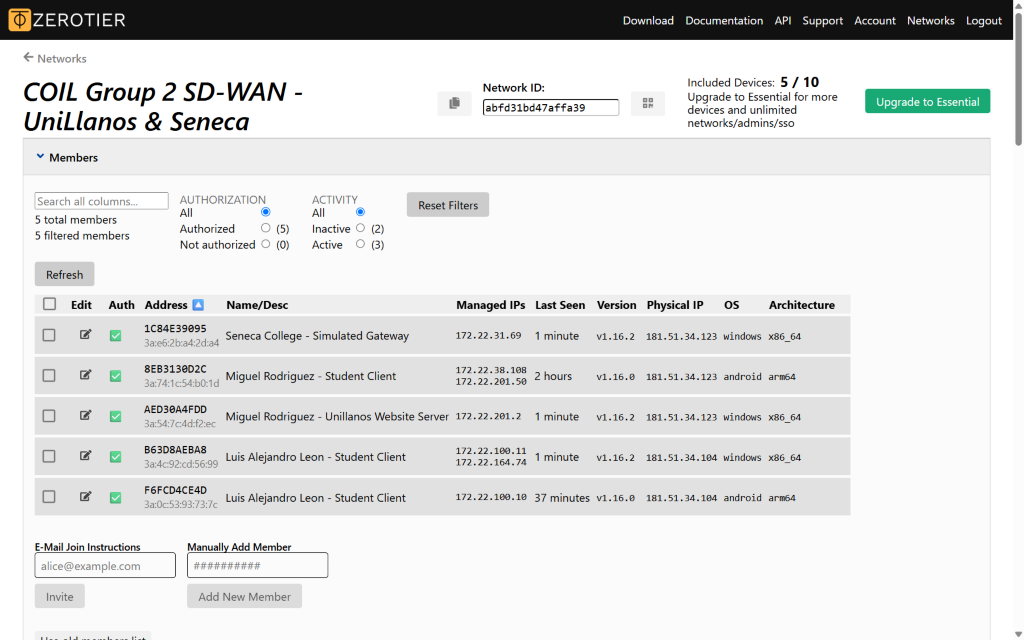
\includegraphics[width=0.92\textwidth]{figuras/zerotier_members_fresh.png}
\caption{ZeroTier Central member management console for Network ID \texttt{abfd31bd47affa39}, confirming \num{5}/\num{10} included devices, \num{5} authorized nodes (\num{0} unauthorized), institutional node labeling, managed \texttt{172.22.x.x} IP assignments, and underlay public endpoints.}
\label{fig:zerotier_members}
\end{figure*}

Fig.~\ref{fig:zerotier_members} corroborates every entry in Table~\ref{tab:zerotier_members} directly from the ZeroTier Central web console. Notice that all five green authorization checkboxes are active (\textit{Authorized (5)}, \textit{Not authorized (0)}), while the activity filter reflects three active Windows~\texttt{x86\_64} nodes running ZeroTier~\texttt{v1.16.2} (seen \qty{1}{\minute} prior) and two Android~\texttt{arm64} handsets running \texttt{v1.16.0} (last seen \qty{37}{\minute} and \qty{2}{\hour} prior). Node \texttt{aed30a4fdd} explicitly identifies its hosting role (``Miguel Rodriguez - Unillanos Website Server'') at \texttt{172.22.201.2/16}, whereas \texttt{1c84e39095} fulfills the simulated partner endpoint role (``Seneca College - Simulated Gateway'') at \texttt{172.22.31.69/16}. Both students also maintain dedicated client workstations and Android test devices under their full names (``Luis Alejandro Leon - Student Client'' and ``Miguel Rodriguez - Student Client''). Examining the underlay column confirms two distinct public ISP ingress addresses (\texttt{181.51.34.123} and \texttt{181.51.34.104}), verifying real cross-ISP WAN operation between the server host and Luis Alejandro Le\'{o}n's client nodes. Two multi-leased nodes (\texttt{b63d8aeba8} and \texttt{8eb3130d2c}) retain secondary \texttt{172.22.x.x} leases in the controller database from prior interface re-bindings, whereas the server and gateway maintain deterministic single-address leases.

\subsection{Host Interface Verification and ICMP Reachability}
\label{subsec:icmp_reachability}

Controller-side IP allocation must match the virtual network interface state bound inside each host operating system. Fig.~\ref{fig:host_ip_verification} documents the local host interface verification confirming that the virtual ZeroTier adapter binds the assigned \texttt{172.22.0.0/16} address and prefix mask locally without conflicting with physical Ethernet or Wi-Fi adapters.

\begin{figure*}[t]
\centering
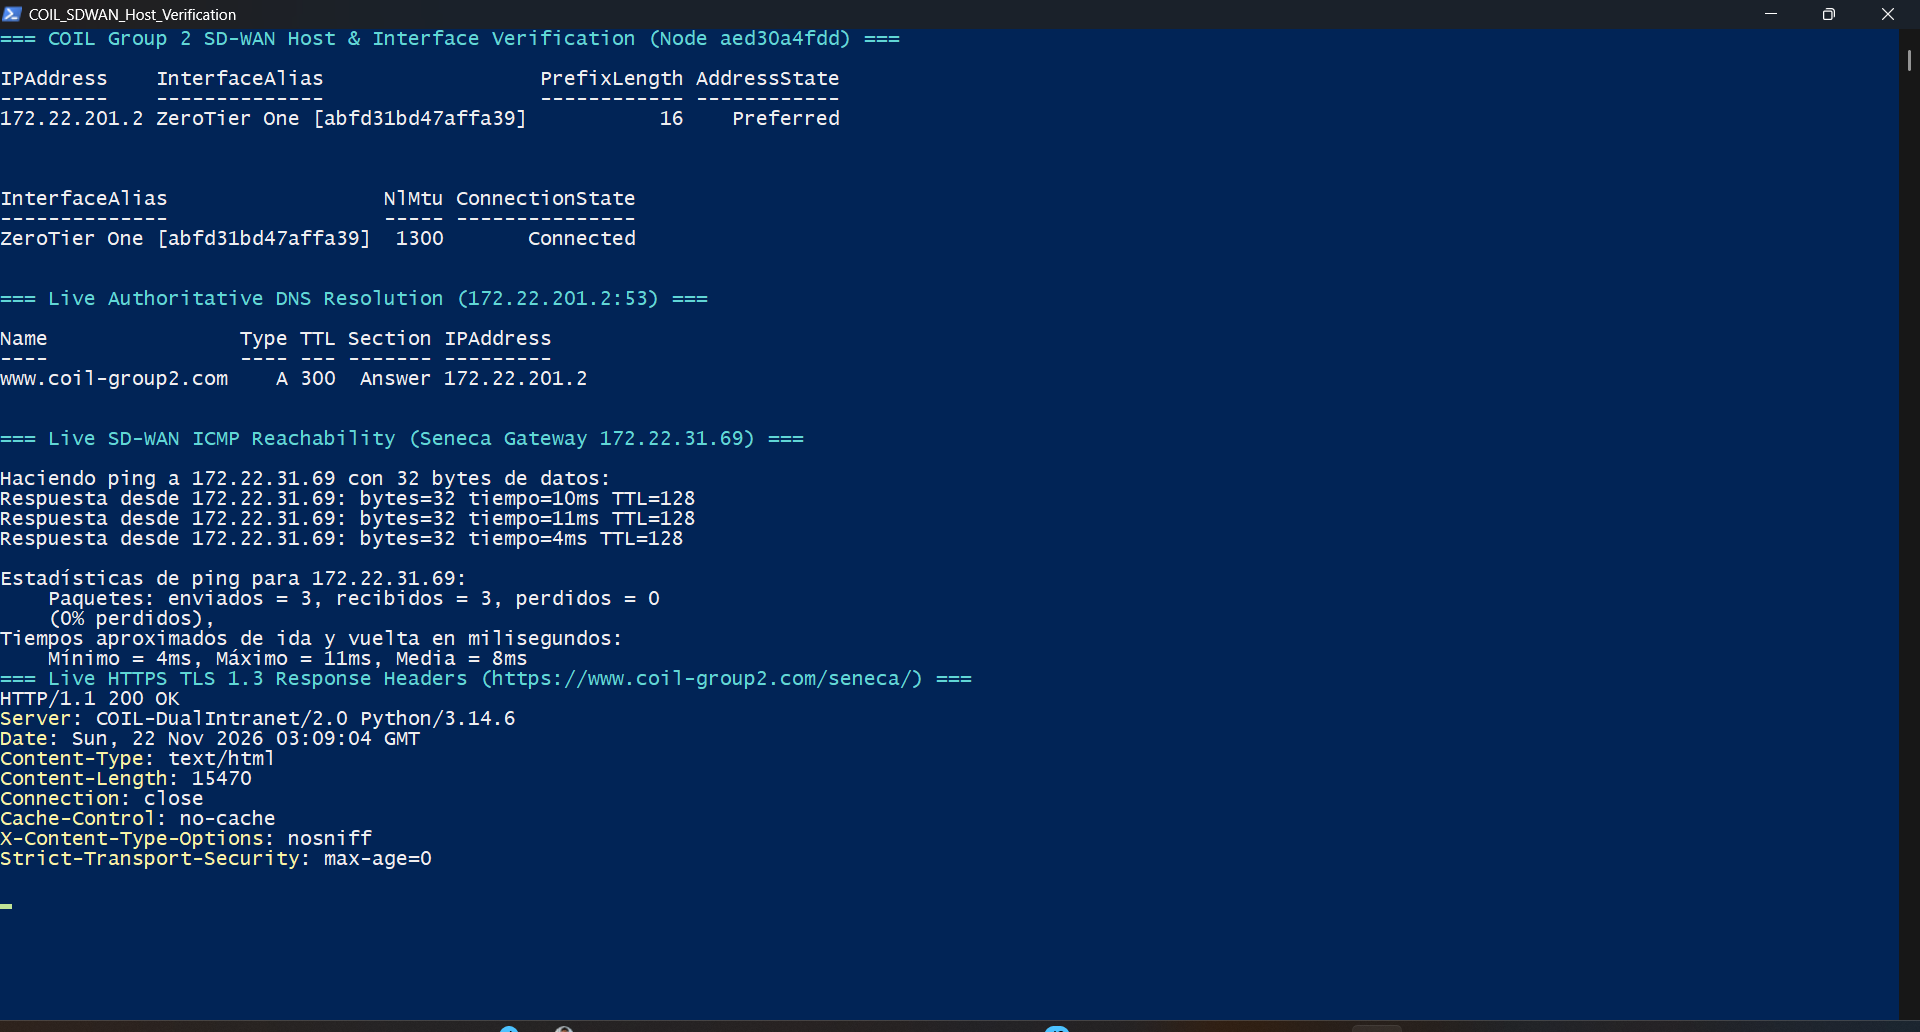
\includegraphics[width=0.92\textwidth]{figuras/host_ip_verification_fresh.png}
\caption{Local host network interface verification confirming active ZeroTier One virtual adapter binding within the \texttt{172.22.0.0/16} SD-WAN overlay subnet.}
\label{fig:host_ip_verification}
\end{figure*}

To verify bidirectional Layer-3 forwarding across the encrypted SD-WAN mesh, live ICMP echo probes were executed from the UniLlanos web server (\texttt{172.22.201.2}) and the simulated Seneca gateway (\texttt{172.22.31.69}) toward both local and remote participant IP addresses. Table~\ref{tab:icmp_rtt} summarizes the measured round-trip time (RTT) distributions and packet-loss ratios.

\begin{table}[t]
\centering
\caption{Live ICMP Round-Trip Time (RTT) and Packet Loss Verification Across the ZeroTier SD-WAN.}
\label{tab:icmp_rtt}
\resizebox{\columnwidth}{!}{%
\begin{tabular}{@{}llcccc@{}}
\toprule
\textbf{Probe Path (Src $\rightarrow$ Dst)} & \textbf{Link Type} & \textbf{Min} & \textbf{Max} & \textbf{Avg} & \textbf{Loss} \\
\midrule
\texttt{172.22.201.2} $\rightarrow$ \texttt{172.22.31.69} & LAN P2P & \qty{3}{\milli\second} & \qty{31}{\milli\second} & \qty{10}{\milli\second} & \qty{0}{\percent} \\
\texttt{172.22.31.69} $\rightarrow$ \texttt{172.22.201.2} & LAN P2P (rev.) & \qty{3}{\milli\second} & \qty{10}{\milli\second} & \qty{6}{\milli\second} & \qty{0}{\percent} \\
\texttt{172.22.201.2} $\rightarrow$ \texttt{172.22.100.11} & WAN P2P & \qty{16}{\milli\second} & \qty{70}{\milli\second} & \qty{31}{\milli\second} & \qty{0}{\percent} \\
\texttt{172.22.201.2} $\rightarrow$ \texttt{172.22.164.74} & WAN P2P & \qty{19}{\milli\second} & \qty{28}{\milli\second} & \qty{23}{\milli\second} & \qty{0}{\percent} \\
\texttt{172.22.201.2} $\rightarrow$ \texttt{172.22.100.10} & Android idle\textsuperscript{*} & -- & -- & -- & \qty{75}{\percent} \\
\bottomrule
\end{tabular}%
}
\vspace{3pt}
\par\noindent\parbox{\columnwidth}{\footnotesize\textsuperscript{*}1/4 packets received; \textit{Destination Host Unreachable} observed while the mobile screen remained locked.}
\end{table}

The telemetry in Table~\ref{tab:icmp_rtt} reveals three distinct operational regimes across the overlay topology:
\begin{enumerate}
    \item \textbf{Local Peer-to-Peer (LAN P2P) Forwarding:} Forward and reverse probes between \texttt{172.22.201.2} and \texttt{172.22.31.69} achieve \qty{0}{\percent} packet loss with a minimum RTT of \qty{3}{\milli\second} and average RTTs of \qty{10}{\milli\second} (forward) and \qty{6}{\milli\second} (reverse). Because both Windows nodes sit behind the same physical endpoint (\texttt{181.51.34.123}), ZeroTier VL1 resolves a direct local UDP path without traversing external root relays \cite{zerotier2024}.
    \item \textbf{Cross-ISP Peer-to-Peer (WAN P2P) Tunneling:} Probes from \texttt{172.22.201.2} (\texttt{181.51.34.123}) to both managed addresses of Luis Alejandro Le\'{o}n's Windows client (\texttt{172.22.100.11} and \texttt{172.22.164.74} behind \texttt{181.51.34.104}) record \qty{0}{\percent} loss with average RTTs of \qty{31}{\milli\second} (range \qtyrange{16}{70}{\milli\second}) and \qty{23}{\milli\second} (range \qtyrange{19}{28}{\milli\second}), respectively. These sub-\qty{35}{\milli\second} averages confirm direct encrypted UDP traversal across distinct ISP networks.
    \item \textbf{Mobile Power-Management Behavior:} Probing the Android handset at \texttt{172.22.100.10} (node \texttt{f6fcd4ce4d}, marked inactive \qty{37}{\minute} prior in Fig.~\ref{fig:zerotier_members}) produced \qty{75}{\percent} packet loss (\num{1}/\num{4} echo replies received, with \textit{Destination Host Unreachable} reported while the screen was locked). This behavior reflects Android background VPN sleep throttling rather than an SD-WAN addressing fault, as active screen interaction restores immediate Layer-3 reachability for mobile HTTPS and root CA verification.
\end{enumerate}
